\chapter{АНАЛИТИЧЕСКАЯ ЧАСТЬ}

В данном разделе будут формализованы задача и данные. Будет разработана ER-диаграмма разрабатываемой системы. Будут проанализированы существующие аналоги. Будут рассмотрены типы пользователей и функционал, который будет им доступен. Будут проанализированы способы организации хранения данных, а также будет выбран наилучший подход к хранению данных для решения поставленной задачи. 

\section{Формализация задачи}\label{data}

Для решения поставленной цели необходимо спроектировать и реализовать базу данных для отображения статистической информации о времени прохождения игр и приложение, которое позволит получать доступ, изменять, добавлять и удалять данные. В базе данных необходимо реализовать три типа ролей: авторизованный пользователь, гость и администратор. 

В базе данных должна храниться информация об: играх, отзывах об играх,
временных отметках о времени прохождения игры, данные для авторизации пользователей, платформах запуска игр, связи между игрой и платформами, на которых запускается игра. 

В таблице \ref{tbl:1} представлены сущности базы данных и их атрибуты.

\captionsetup{justification=raggedleft,singlelinecheck=off}
\begin{table}[H]
	\centering
	\caption{Категории и сведения о данных}
	\label{tbl:1}
	\begin{tabular}{|l|l|}
		\hline
		\textbf{Сущность}                                                                   & \textbf{Атрибуты}                                                                                                                                       \\ \hline
		Игры                                                                               & \begin{tabular}[c]{@{}l@{}}ID игры, название игры, дата выхода,\\ разработчик, издатель, жанры\end{tabular}                                         \\ \hline
		Временная отметка                                                                          & \begin{tabular}[c]{@{}l@{}}ID игры, имя пользователя, количество ча-\\сов, количество минут, тип прохождения.\\\end{tabular} \\ \hline
		Отзыв                                                            & \begin{tabular}[c]{@{}l@{}} ID игры, имя пользователя, текст отзыва, \\оценка, дата публикации.  \\\end{tabular}                                                                                                                  \\ \hline
		Пользователь                                                                           & \begin{tabular}[c]{@{}l@{}}Имя пользователя, пароль.\end{tabular}                                                                                                      \\ \hline
		Платформа                                                                         & \begin{tabular}[c]{@{}l@{}}ID платформы, название, средняя стоимость \\\end{tabular}                                   \\ \hline
		Связь платформ и игр                                                                 & ID платформы, ID игры.                                                                                                                 \\ \hline
	\end{tabular}
\end{table}


Согласно таблице \ref{tbl:1}, на рисунке \ref{img:er} изображена ER-диаграмма базы данных.

\begin{figure}[H]
	\begin{center}
		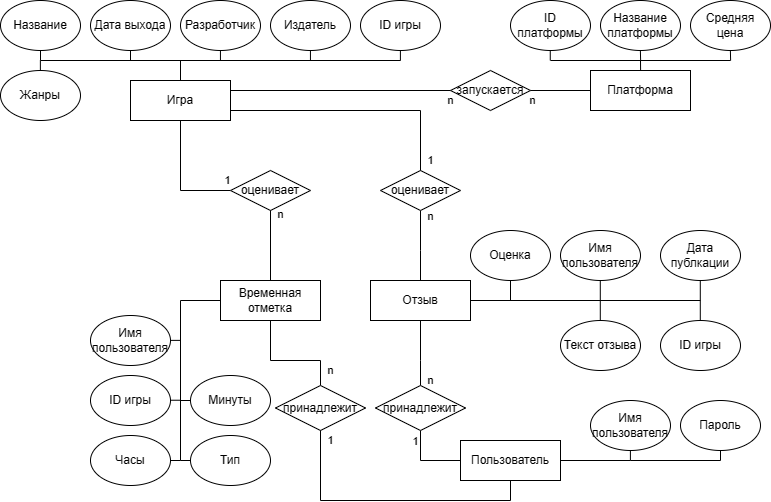
\includegraphics[scale=0.6]{../imgs/er.png}
	\end{center}
	\captionsetup{justification=centering}
	\caption{ER-диаграмма}
	\label{img:er}
\end{figure}

\section{Типы пользователей и доступная им функциональность}\label{functions}

Одной из задач курсовой работы является разработка приложения, котором будет возможность авторизации. Таким образом, необходимо разработать ролевую модель, состоящую из авторизованных пользователей, неавторизованных пользователей (гостей) и администраторов.

Каждый тип пользователя имеет свою специфическую функциональность, которая может быть описана с помощью диаграмм прецедентов (Use Case диаграммы). 

Набор функций, которые могут быть использованы неавторизованными пользователями:
\begin{itemize}
	\item[---] аутентификация,
	\item[---] регистрация,
	\item[---] просмотр различной статистики о времени прохождения игры по разным категориям,
	\item[---] просмотр отзывов и оценок,	
	\item[---] просмотр информации об игре. 
\end{itemize}

На рисунке \ref{img:ucguest} представлена Use case диаграмма для неавторизованного пользователя.
\begin{figure}[H]
	\begin{center}
		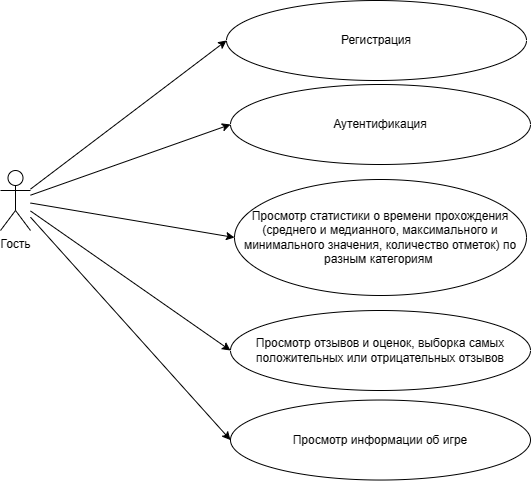
\includegraphics[scale=0.8]{../imgs/guest.png}
	\end{center}
	\captionsetup{justification=centering}
	\caption{Диаграмма прецедентов для неавторизованного пользователя}
	\label{img:ucguest}
\end{figure}
	
Набор функций, которые могут быть использованы авторизованными пользователями:
	\begin{itemize}
		\item[---] просмотр информации об игре,
		\item[---] просмотр различной статистики о времени прохождения игры по разным категориям,
		\item[---] добавление отзывов и оценок,
		\item[---] добавление информации о времени прохождения игры,
		\item[---] просмотр отзывов и оценок,	
		\item[---] выход. 
	\end{itemize}

На рисунке~\ref{img:ucuser} представлена Use case диаграмма для неавторизованного пользователя.

\begin{figure}[H]
	\begin{center}
		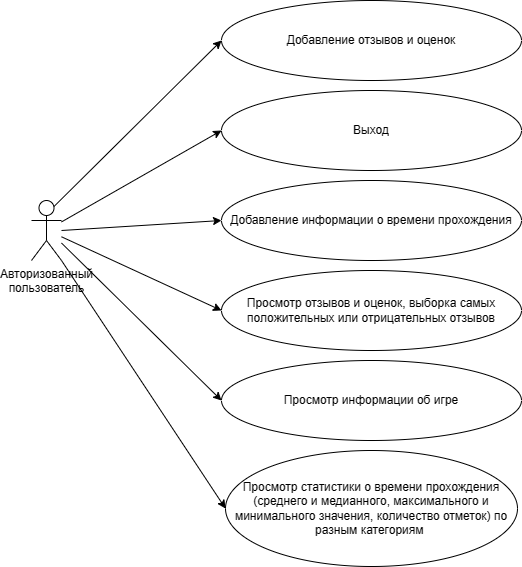
\includegraphics[scale=0.8]{../imgs/user.png}
	\end{center}
	\captionsetup{justification=centering}
	\caption{Диаграмма прецедентов для авторизованного пользователя\\}
	\label{img:ucuser}
\end{figure}

Набор функций, которые могут быть использованы администратором:
	\begin{itemize}
		\item[---] выход,
		\item[---] просмотр и изменение, добавление, удаление всей информации, доступной в базе данных.
	\end{itemize}

На рисунке~\ref{img:ucadmin} представлена Use case диаграмма для администратора.

\begin{figure}[h!]
	\begin{center}
		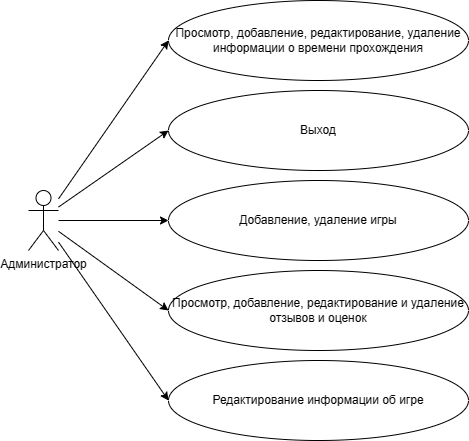
\includegraphics[scale=0.8]{../imgs/admin.png}
	\end{center}
	\captionsetup{justification=centering}
	\caption{Диаграмма прецедентов для администратора}
	\label{img:ucadmin}
\end{figure}


\section{Анализ существующих аналогов}\label{criteria}

Для того чтобы проанализировать существующие аналогичные решения, были определены следующие критерии:

\begin{enumerate}
	\item Возможность указать время прохождения игры;
	\item Возможность оставлять оценки и отзывы;
	\item Наличие интерфейса на русском языке.
\end{enumerate}

Steam~\cite{steam} --- один из самых популярных магазинов видео игр. Он позволяет не только покупать игры, но и оставять обзоры на них. Также Steam считает время проведенное в игре, но не может собирать информацию времени прохождения~(рисунок~\ref{fig:steamex}). Имеет русский интерфейс.

\begin{figure}[H]
	\centering
	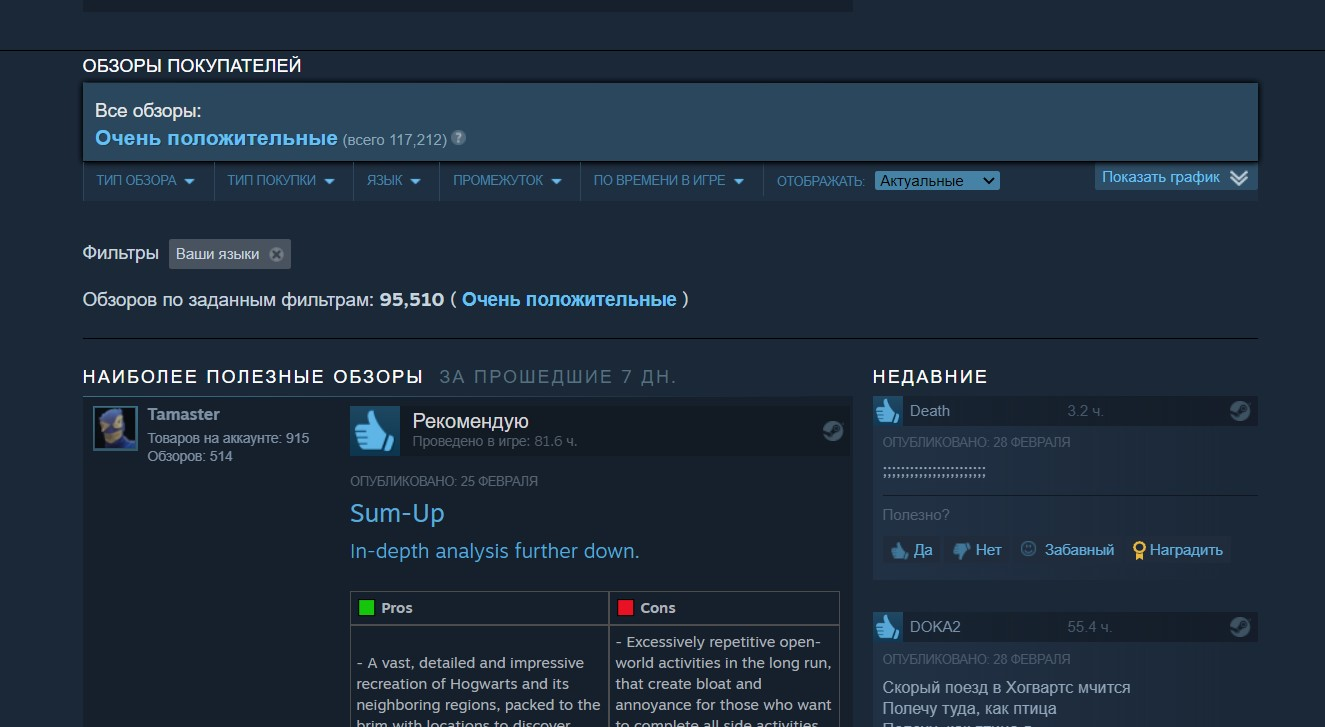
\includegraphics[width=0.7\linewidth]{../imgs/steam_ex}
	\captionsetup{justification=centering}
	\caption{Приложение Steam}
	\label{fig:steamex}
\end{figure}

HowLongToBeat~\cite{hltb} --- cайт, на котором можно оставлять обзоры и оценки видеоигр, а также оставлять время прохождения игры по 2 категориям: основной сюжет, 100\% прохождение~(рисунок~\ref{fig:hltbex}). Данный сайт имеет серьезный недостаток, он полностью на английском языке.
\clearpage
\begin{figure}[H]
	\centering
	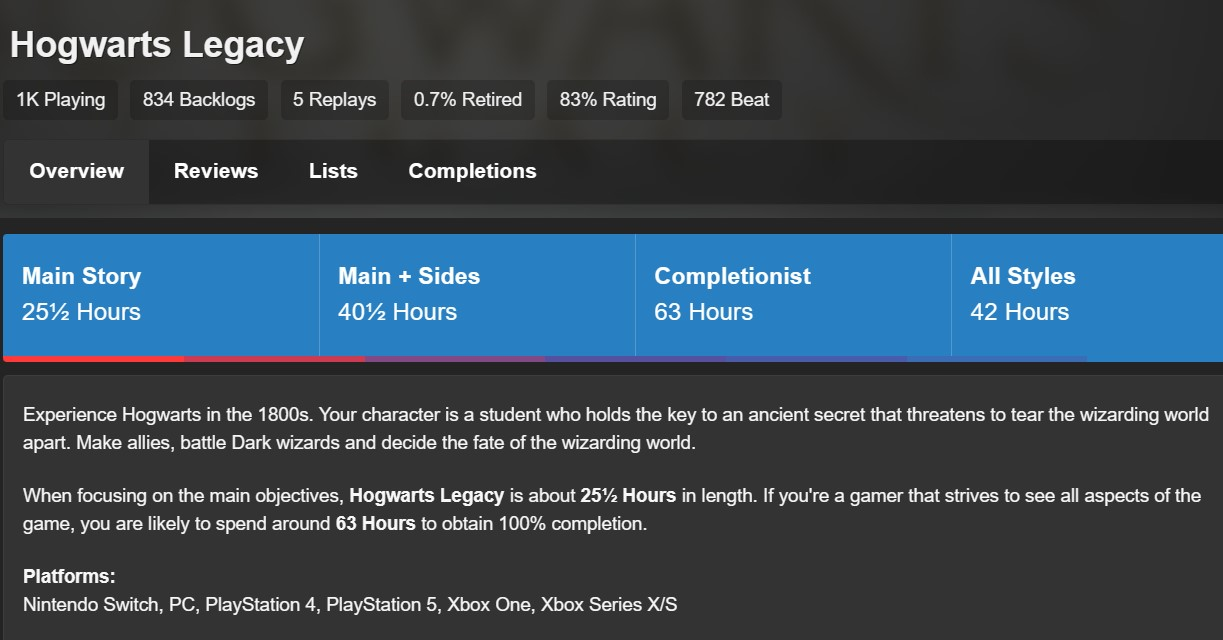
\includegraphics[width=0.7\linewidth]{../imgs/hltb_ex}
	\captionsetup{justification=centering}
	\caption{Сайт HowLongToBeat}
	\label{fig:hltbex}
\end{figure}

В таблице~\ref{tbl:2} сравниваются существующие аналоги в соответствии с критериями, перечисленными в пункте~\ref{criteria}. В таблице приняты следующие обозначения: время прохождения --- возможность указать время прохождения игры, отзывы и оценки ---  возможность оставлять оценки и отзывы, русский язык --- наличие интерфейса на русском языке.

~

\captionsetup{justification=raggedleft,singlelinecheck=off}
\begin{table}[H]
	\centering
	\caption{Сравнение существующих аналогов}
	\label{tbl:2}
	\begin{tabular}{|l|l|l|l|}
		\hline
		Сервис & Время прохождения & Отзывы и оценки  & Русский язык \\ \hline
		Steam & - & + & +  \\ \hline
		HowLongToBeat & +  & + & - \\ \hline
	\end{tabular}
\end{table}

~

Таким образом, ни одно из существующих решений не обладает всеми функциями, которые должны быть реализованы в разрабатываемом приложении. В частности, Steam не позволяет посмотреть среднее время игры, а HowLongToBeat не имеет русского интерфейса.

~

~

\section{Анализ существующих видов баз данных} 

Для решения поставленной цели необходимо разработать базу данных (БД). БД --- это упорядоченный набор структурированной информации или данных, которые обычно хранятся в электронном виде в компьютерной системе~\cite{database}.

\subsubsection{Классификация реляционных баз данных по способу хранения}

Реляционные базы данных по способу хранения делятся на две группы: строковые и колоночные.\\

\noindent\textbf{Строковые базы данных}

Строковые базы данных, в которых записи хранятся построчно, в основном используются в транзакционных системах(англ. \texttt{OLTP} \cite{OLTP}), характеризующихся большим количеством коротких операций вставки, обновления и удаления. OLTP-системы лучше всего для быстрой обработки запросов и поддержания целостности данных в средах с множественным доступом.\\

\noindent\textbf{Колоночные базы данных}

Колоночные базы данных - это базы данных, в которых записи хранятся в "колонках". Этот тип в основном используется в аналитических системах (\texttt{OLAP} \cite{olap}), характеризующихся низкими объемами транзакций и запросами, которые часто бывают сложными и включают агрегирование. Мерой эффективности таких систем является время ответа. Наличие агрегированных исторических данных позволяет системам OLAP применять интеллектуальные аналитические методы.

\subsection{Кэширование данных}

Чтобы уменьшить время отклика, можно использовать механизм кэширования данных, для реализации которого подходят \texttt{NoSQL} \cite{nosql} \texttt{in-memory} базы данных, хранящие данные в оперативной памяти, что обеспечивает более быстрый доступ, по сравнению с традиционными реализациями.

Для сокращения времени отклика можно использовать механизм кэширования данных, который может быть реализован с помощью \texttt{NoSQL} \cite{nosql} \texttt{in-memory} базы данных, которые обеспечивают более быстрый доступ, чем традиционные приложения, за счет хранения данных в оперативной памяти.

\noindent\textbf{Проблема синхронизации данных}

Приложение записывает данные в кэш и базу данных, но они никак не синхронизированы, что приводит к несоответствиям в данных. Например, может возникнуть ситуация, когда данные удаляются из хранилища и одновременно должны быть удалены из кэша. Эту проблему можно решить с помощью создания триггеров. Триггеры могут запускать изменения или удаления и синхронизировать данные в кэше.

\noindent\textbf{Проблема <<холодного старта>>}

Когда кэш создается впервые, он пуст и не содержит никаких данных. Все запросы отправляются непосредственно в базу данных, и только через некоторое время кэш содержит необходимую информацию. При перезапуске предыдущее состояние кэша может быть восстановлено из журнала событий, хранящегося на диске. При перезапуске кэша данные должны быть синхронизированы с хранилищем - может оказаться, что некоторые данные в кэше устарели на момент перезапуска.


